\section{Model to Develop}

The aim of this internship is to develop a machine learning model that provides as output (\textbf{Y}) a regional-scale, high-resolution weather forecast, which will be referred to as High Resolution Local (\textbf{HRL}) in this document. Initially, the input (\textbf{X}) will be an HRL at time t, denoted as \textbf{HRL(t)}. This first model will represent a simple forecast. Subsequently, a low-resolution global model, referred to as Low Resolution Global (\textbf{LRG}), will be added to the input to potentially improve the system's predictions by providing context.

The work of \href{https://events.ecmwf.int/event/172/contributions/1769/attachments/877/1550/Machine-Learning-WS_Mdini.pdf}{Maha Mdini} should be analyzed to identify any ideas that could be incorporated into the future model.

\vspace{2em}

\begin{tabular}{>{\bfseries}l<{\hspace{1em}} >{\centering\arraybackslash}p{7cm} >{\raggedleft\arraybackslash}p{2cm}}
\hline
\textbf{Model to Develop} & \textbf{Input (X)} & \textbf{Output (Y)}\\
\hline
Model 1 & HRL(t) & HRL(t+dt) \\
Model 2 &  HRL(t) + LRG(t) & HRL(t+dt) \\
Model 3 &  HRL(t) + LRG(t) + LRG (t+dt) & HRL(t+dt) \\
Model 4 & autoregressive & HRL(t+dt) \\
\end{tabular}

\subsection{Model 1: Simple Forecast within a Region}

\begin{figure}[ht]
\centering
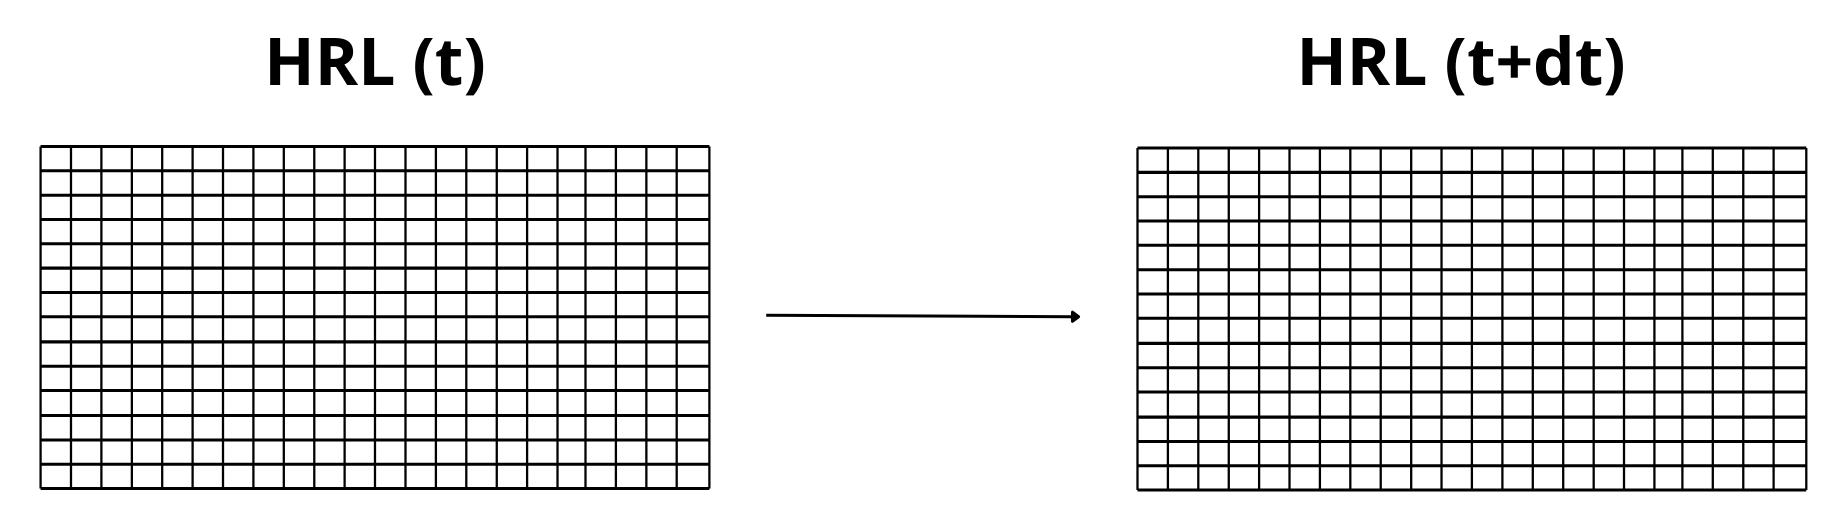
\includegraphics[width=0.9\textwidth]{media/model1.png}
\caption{Architecture of Model 1: Simple Forecast}
\label{fig}
\end{figure}

This model represents a simple forecast within a region with a known state at time t on a fine grid to obtain a known state at time t+dt on a fine grid.

\subsection{Model 2: Forecast with Boundary Conditions}

\begin{figure}[ht]
\centering
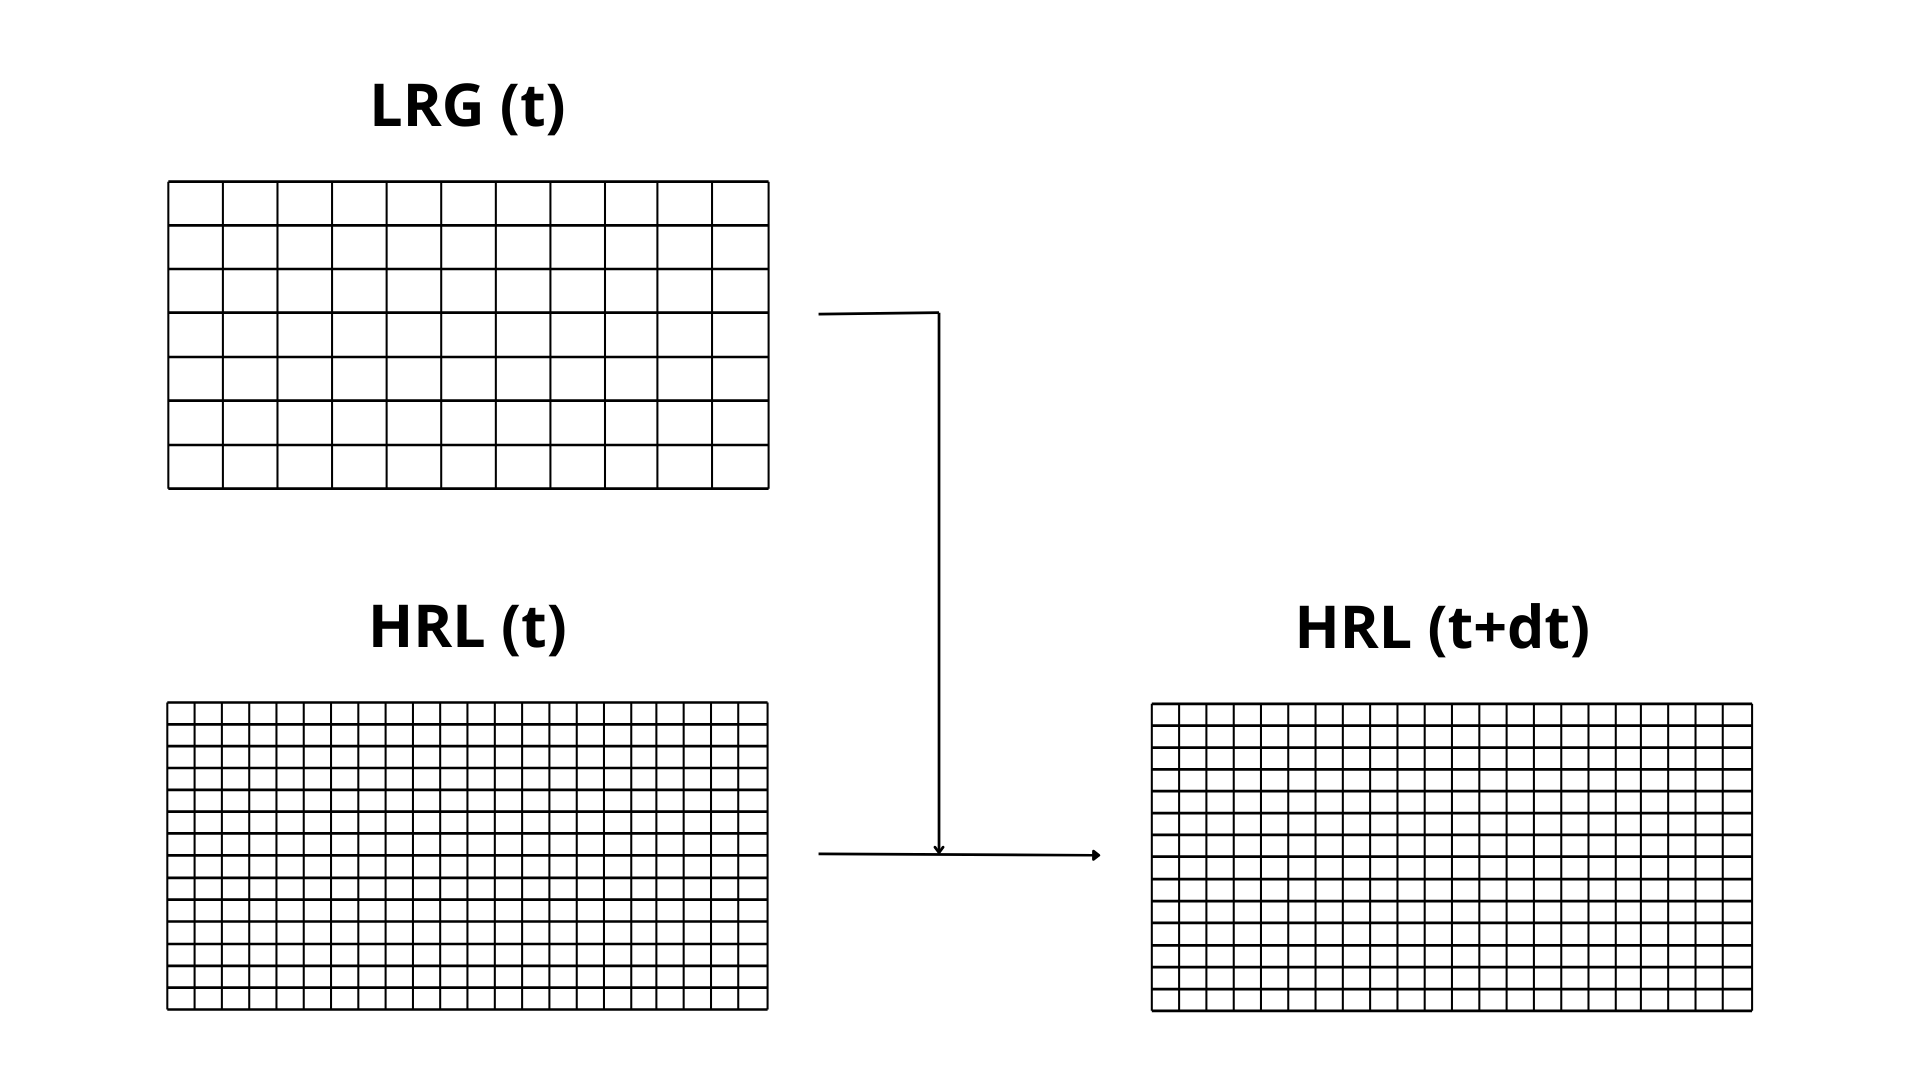
\includegraphics[width=0.9\textwidth]{media/model2.png}
\caption{Architecture of Model 2: Forecast with Degraded Boundary Conditions}
\label{fig}
\end{figure}

The objective of this model is to test whether having a broader system state at time t (boundary conditions) with lower resolution can yield better results for the local high-resolution domain at time t+dt.

\subsection{Model 3: Forecast and Downscaling}

\begin{figure}[ht]
\centering
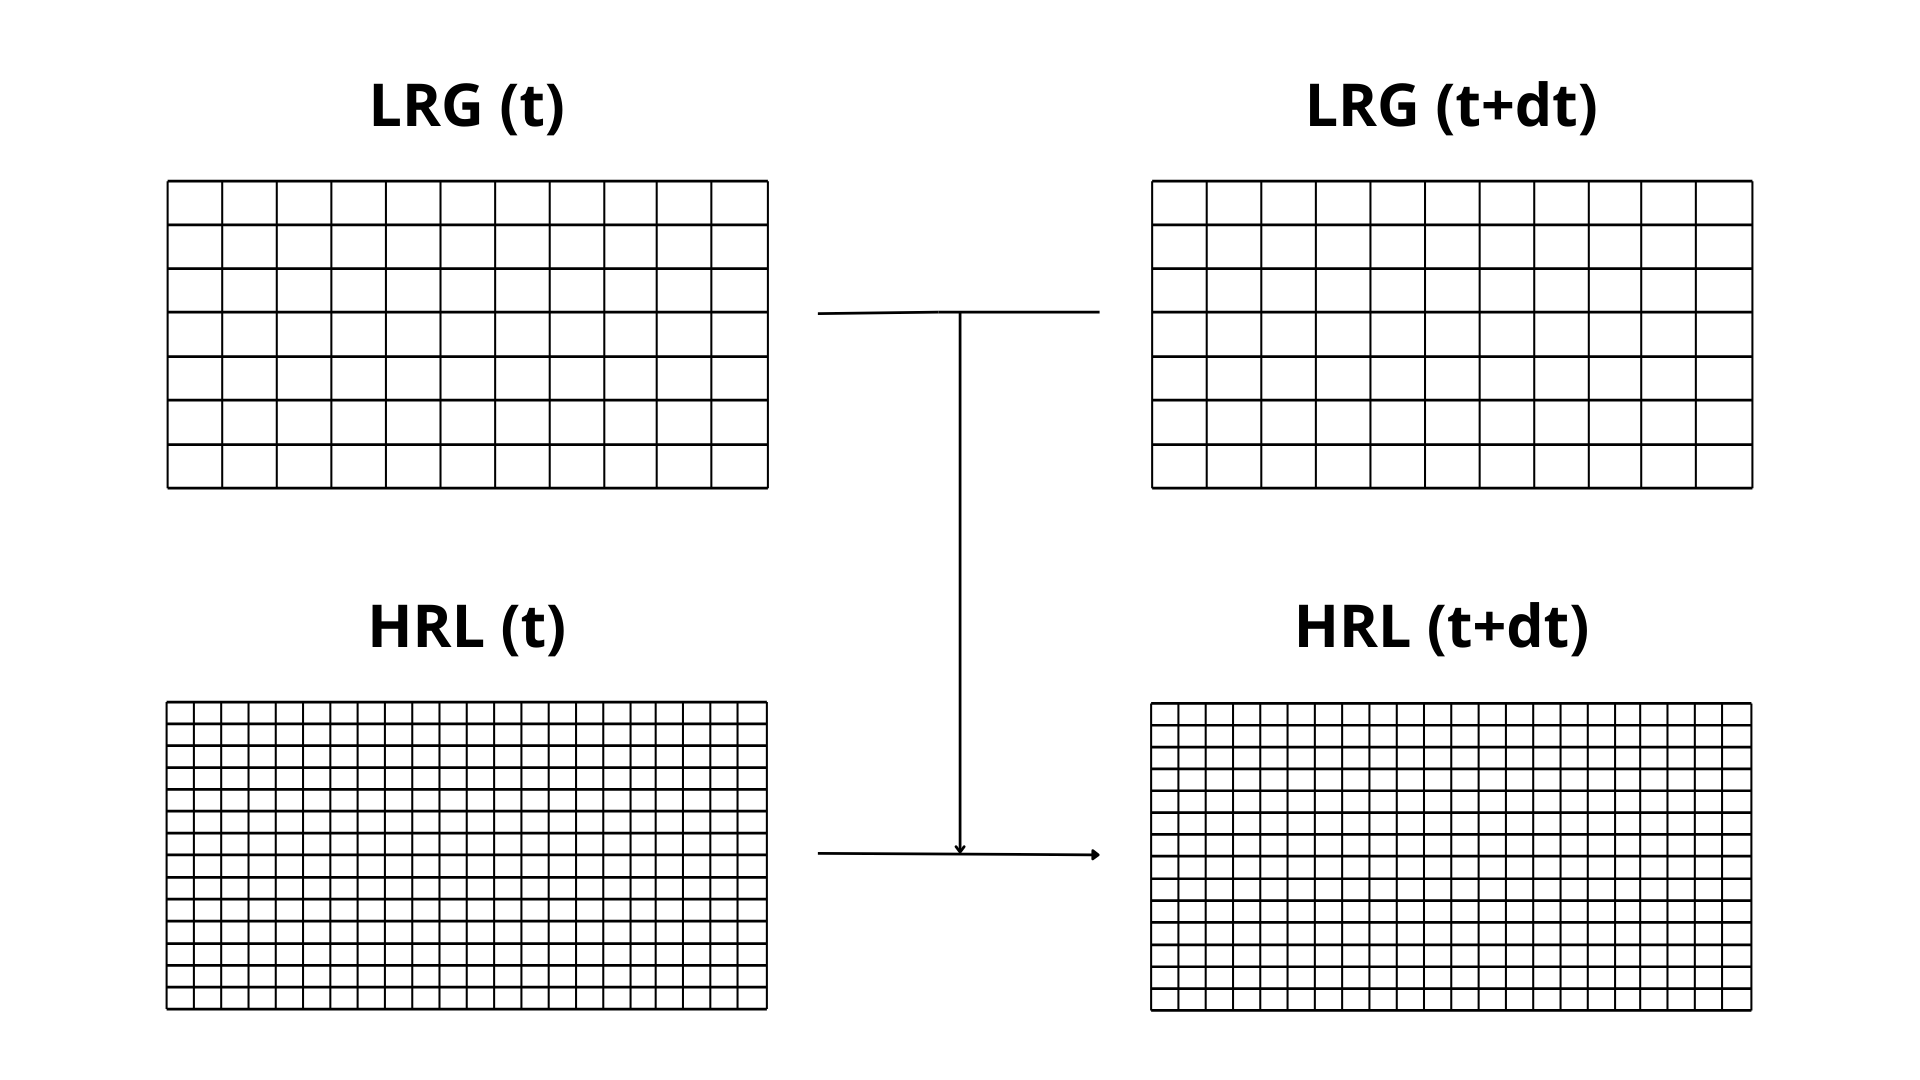
\includegraphics[width=0.8\textwidth]{media/model3.png}
\caption{Architecture of Model 3: Forecast and Downscaling}
\label{fig}
\end{figure}

The objective of this model is to test whether having a broader system state at both time t and time t+dt (the predicted time) with lower resolution can yield better results for the local high-resolution domain at time t+dt. This model involves both forecasting and downscaling steps.

\subsection{Model 4: Rollout or Autoregressive}

\begin{figure}[ht]
\centering
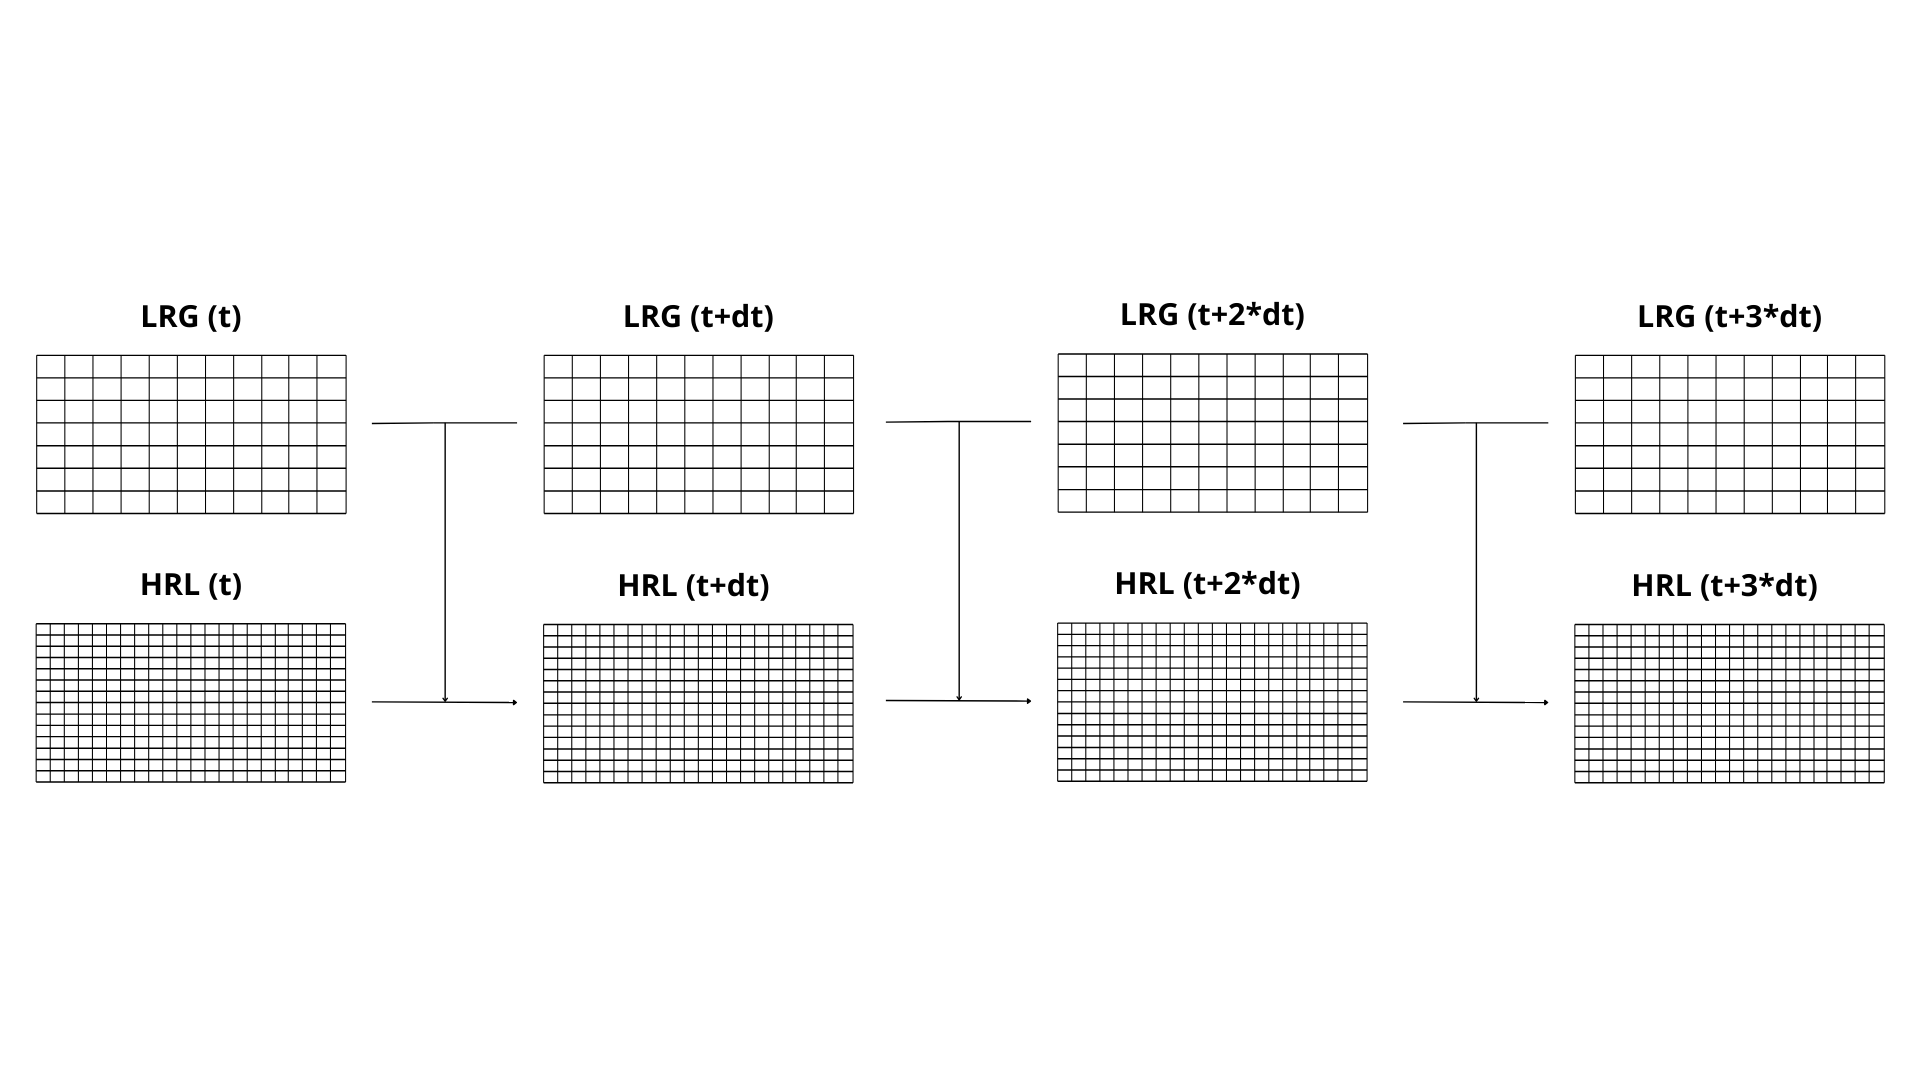
\includegraphics[width=0.9\textwidth]{media/model4.png}
\caption{Architecture of Model 4: Rollout}
\label{fig}
\end{figure}

The output from the previous iteration becomes the new input. The goal is to test the model's ability to predict an output at time n without significant error accumulation.